\section{Definitions and Nomenclauture}
\label{sec:definitions}

In order to define stable learning algorithms, it is imperative to first recall the definition of first-order systems and stability, which is taken from \cite{khalil_nonlinear_2002}.

\begin{definition}[System]
    A continuous-time first-order system is defined by the following map
       \begin{equation}
       f:\mathbb{R}^n\times\mathbb{R}^m\rightarrow \mathbb{R}^n, (x(t),u(t)) \mapsto \dot x(t) = f(x(t),u(t)).
       \label{def:eq-system}
       \end{equation}
   
       Additionally, if $u(t)$ is a function of $x$, the system is considered autonomous, with closed-loop dynamics $f(x(t))$. The trajectory of the system is defined by the evolution of $x(t)$. Furthermore, the system has an equilibrium point at $f(x(t))=0$.
       \label{def:system}
   \end{definition}
   
   \begin{definition}[Stability]
    Consider the equilibrium point $x=0$ of \eqref{def:eq-system}. Then the system is:
    \begin{itemize}
    \item \textit{stable}, if for each $\epsilon>0$, there is a $\delta>0$, such that
        $$||x(0)||<\delta \Rightarrow ||x(t)||<\epsilon, \quad \forall t \geq 0$$ 
    \item \textit{unstable}, if not stable, and
    \item \textit{asymptotically stable} if it is stable and $\delta$ can be chosen such that
        $$||x(0)||<\delta \Rightarrow \lim_{t\rightarrow\infty} x(t)=0 $$
    \end{itemize} 
   \end{definition}
   Henceforth, the dependency of the dynamics on time is considered to be implicit and will be neglected in the notation.
   
   
   \begin{definition}[Lyapunov function]
    A Lyapunov function is a continuous function $V: \mathbb{R}^n\rightarrow\mathbb{R}$ with the following properties:
    \begin{enumerate}
     \item[(a)] \textit{positive definiteness}, $V(x)>0 \quad \forall x\in\mathbb{R}^n\setminus\{0\}$ and $V(0)=0$,
     \item[(b)] \textit{decrease condition}, $\dot V(x)\leq0 \quad \forall x\in\mathbb{R}^n$.
    \end{enumerate}
    \label{def:lyapunov-function}
   \end{definition}
   
   \begin{definition}[Lyapunov stability]
       A system of the form \eqref{def:eq-system} is said to be \textit{Lyapunov stable}, if there exists a function $V(\cdot)$ that satisfies the conditions of Definition \ref{def:lyapunov-function}a and \ref{def:lyapunov-function}b.
       \label{def:lyapunov-stability}
   \end{definition}
   
   The ultimate goal of this work is to develop stable update laws for NNCs. Hence, the designed control law will be considered as a NN. Therefore, the following definition of NNs is used throughout this work.
   
   \begin{definition}[Neural network]
    A feedforward neural network (NN) $\phi:\mathbb{R}^n\rightarrow \mathbb{R}^m$ is defined as:
   \begin{equation}
    \begin{aligned}
    \phi (x) & = (L_{H} \circ \varphi_{H} \dots \circ L_{2} \circ \varphi_{2} \circ L_{1} \circ \varphi_1)(x)\\
    L_i(x) &= \theta_i x + b_i \quad \forall i\in\{1,..., H\},
   \end{aligned}
   \end{equation}
    where the activation functions are called $\varphi_i(\cdot)$, $\theta_i$ and $b_i$ are the weight matrix and bias of layer $i$, respectively. Whenever a bias is not mentioned it is assumed to be zero.
\end{definition}

NNs usually make use of nonlinear activation functions, which enable them to approximate nonlinear functions. Throughout this work, an activation function that is designed to model a smooth saturation function is used, as done in \cite{wahby_enhanced_2024} and defined as follows:
\begin{equation}
 \sigma (x;a_{sat}) = \frac{2(1-e^{-a_{sat}x})}{a_{sat}(1+e^{-a_{sat}x})}
 \label{eq:sigmoid}
\end{equation}
Note that the activation function saturates at $\pm \frac{2}{a_{sat}}$. Henceforth, the saturation function is denoted as $\sigma(x)$ and is applied elementwise.

\hl{Define LQR??}


\section{Methodology}
\subsection{Nonlinear Model Reference Adaptive Control}
\begin{theorem}
    The function constitutes a Lyapunov function:
    \begin{equation}
    V(e,\theta) = ||e||_P^2 + ||\alpha(e_x,\theta)||_{\Gamma^{-1}}^2
    \end{equation}

\end{theorem}


The system is defined as in equation \eqref{eq:mimo-system}. Furthermore, we define a reference model that imposes a desired behavior on the system, as defined in equation \eqref{eq:mimo-ref}. Note, that we assume $A,A_m\in\mathbb{R}^{n \times n}$, $B,B_m\in\mathbb{R}^{n\times m}$, $\theta,\theta_m\in\mathbb{R}^{m\times n}$, and $\phi, \phi_m$ are applied element-wise.

\begin{equation}
 \dot x = Ax + B\phi(\theta e_x), \quad e_x = r-x
    \label{eq:mimo-system}
\end{equation}

\begin{equation}
 \dot x_m = A_mx_m + B_m\phi_m(\theta_m e_m) \quad e_m = r-x_m
    \label{eq:mimo-ref}
\end{equation}

We define the internal error of the system with respect to the model reference $e=x_m-x$, which results in the time derivative of the error to be as defined in equation \eqref{eq:e_dot_mimo}. 

\begin{equation}
    \begin{aligned}
 \dot e  = & \dot x_m - \dot x \\
         = &  A_mx_m + B_m\phi_m(\theta_m e_m) \\ 
        & - \left[Ax + B\phi(\theta e_x)\right] \pm \left[A_mx + B_m\phi_m(\theta_m e_x)\right] \\
         = & A_m e + \underbrace{B_m\phi_m(\theta_m e_m) - B_m\phi_m(\theta_m e_x)}_{:=\gamma_m(e_m,e_x)} \\
        & + \underbrace{(A_m-A)x + B_m\phi_m(\theta_m e_x) - B\phi(\theta e_x)}_{:=\alpha(e_x,\theta)}\\
        = & A_m e + \gamma_m(e_m,e_x) + \alpha(ex_, \theta)
    \end{aligned}
    \label{eq:e_dot_mimo}
\end{equation}
Note, that the term $\alpha$ describes the difference in the dynamics.

The following Lyapunov candidate is defined:
\begin{equation}
    V(e,\theta) = ||e||_P^2 + ||\alpha(e_x,\theta)||_{\Gamma^{-1}}^2
    \label{eq:lyapunov-candidate-mimo}
\end{equation}
Here $P,\Gamma^{-1}\in\mathbb{R}^{n\times n}$ are positive definite matrices. Note, that the Lyapunov function consists of the squared norm of the error $e$, and the squared norm of the difference in dynamics $\alpha(e_x,\theta)$, rendering the Lyapunov function to be positive definite. Hence, this function can only be equal to zero, when the internal error and the differnce in dynamics are exactly equal. Additionally, showing the negative definitness of its time derivative results in stability of the closed-loop system during the learning process.

Its time derivative is given by \eqref{eq:lyapunov-candidate-mimo-dot}.

\begin{equation}
    \begin{aligned}
        \dot V(e,\theta) = &  \dot e^T P e + e^T P \dot e \\
        & + \dot\alpha(e_x,\theta)^T\Gamma^{-1}\alpha(e_x,\theta)\\ 
        & + \alpha(e_x,\theta)^T\Gamma^{-1}\dot\alpha(e_x,\theta)\\
        = & \underbrace{-e^T(A_m^TP + PA_m)e^T}_{\textrm{(I)}} \\
        & + \underbrace{2e^TP\gamma(e_m,e_x)}_{\textrm{(II)}} \\
        & + \underbrace{2\alpha(e_x,\theta)^T(Pe+\Gamma^{-1}\dot\alpha(e_x,\theta))}_{\textrm{(III)}}\\
    \end{aligned}
    \label{eq:lyapunov-candidate-mimo-dot}
\end{equation}

Following the logic of linear MRAC, term $\textrm{(III)}$ is used to define the update law through nullification. Hence, it remains to show that the sum of terms $\textrm{(I)}$ and $\textrm{(II)}$ are negative. The negative definiteness of these two terms are system dependent. \hl{In} \cref{sec:results}, we will show that there exists at least one system, where the sum of terms remains negative. To continue with the derivation of the update law, we will for now assume that the sum of these two terms remain negative.

To derive the MIMO update law, we require term $\textrm{(III)}$ in \cref{eq:lyapunov-candidate-mimo-dot} to be equal to zero. Since, $\Sigma=B \frac{\partial \phi(\tilde x)}{\partial \tilde x}\vert_{\tilde x=\theta e_x}\in\mathbb{R}^{n\times m}$, the matrix is not invertible. Therefore, its Moore-Penrose inverse is defined as $\Sigma^{\dagger}$.

\begin{equation}
    \begin{aligned}
        \Rightarrow \dot\theta e_x = \Sigma^{\dagger}
        \biggl[ &\Gamma Pe \\
           + & (A_m-A)\dot x + B_m \frac{\partial \phi_m(\tilde x)}{\partial \tilde x}\vert_{\tilde x=\theta_m e_x}\theta_m \dot e_x \\
           - & B \frac{\partial \phi(\tilde x)}{\partial \tilde x}\vert_{\tilde x=\theta e_x}\theta \dot e_x \biggr]
    \end{aligned}
    \label{eq:moore-penrose2}
\end{equation}
Henceforth, for shorter notation the term in big square brackets will now be called $\xi$.

Recall, $\dot\theta\in\mathbb{R}^{m\times n}$, $e_x \in\mathbb{R}^{n}$, $\Sigma^{\dagger}\in\mathbb{R}^{m\times n}$, $\xi\in\mathbb{R}^{n}$, and we desire to solve for $\dot\theta$. The solution of this equation is given by equation \eqref{eq:MIMO-update-law}, which corresponds to the MIMO nonlinear MRAC update law. Note, $e_x^{\dagger}$ is the pseudo-inverse of $e_x$, which is defined as $e_x^{\dagger}=0$, if $e_x=0$, and $e_x^{\dagger}=e_x^T(e_x^Te_x)^{-1}$ otherwise.

\begin{equation}
\dot\theta =\Sigma^{\dagger}\xi e_x^{\dagger}
    \label{eq:MIMO-update-law}
\end{equation}

This system of equations always has an infinite number of solutions, except if  $e_x=0$, and simultaneously $\Sigma^{\dagger}\xi\neq 0$. Whenever, this case occurs, we propose to not update the weights of the neural network. However, when there is an infinite number of solutions, we can choose values for $\dot\theta$, that satisfy this equation. For example, we could choose the solution that minimizes the spectral norm of $\dot\theta$. The idea is based on \cite{yoshida2017spectralnormregularizationimproving, johansson_improved_2023}, where it was proposed to minimize the spectral norm of the Jacobian of the NN, to improve its robustness properties. In our case, this would correspond to taking the solution, where $\dot\theta$ has the smallest maximum singular value. By minimizing the norm, we ensure that no direction in the weight space undergoes excessively large changes during training. This can help in preventing sudden changes of $\theta$, and aid towards a more smooth learning process.

\subsection{System Model}
\label{sec:system}
The proposed method is simulated and implemented on a sea-saw-like system, as shown in \cref{fig:flying-arm}. 
% The resulting blockdiagram is shown in \cref{fig:blockdiagram-double-flying-arm}.

\begin{figure}
    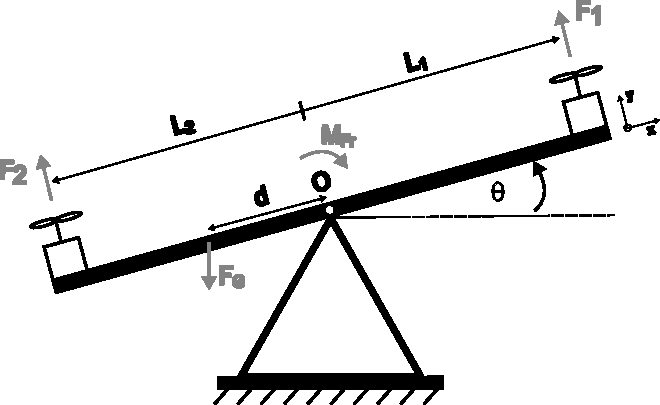
\includegraphics[width=\linewidth]{images/DoubleFlyingArm.pdf}
    \caption{Double flying arm}
    \label{fig:flying-arm}
\end{figure}

% \begin{figure}[h]
%     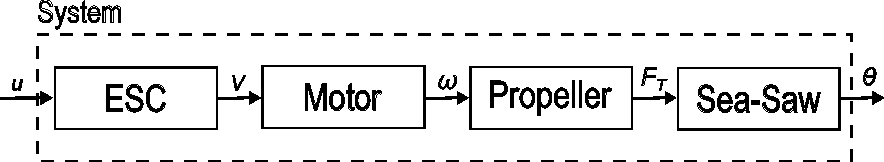
\includegraphics[width=0.8\textwidth]{images/DoubleFlyingArm_Blockdiagram.pdf}
%     \caption{\hl{Blockdiagram of the double flying arm}}
%     \label{fig:blockdiagram-double-flying-arm}
% \end{figure}

The dynamics of the system are given by the following:
\begin{equation}
    \ddot\theta = \frac{1}{J}(L_1F_1-L_2F_2-f_r\dot\theta-d\cos(\theta)F_{G})
    \label{eq:dyn-double-flying-arm}
\end{equation}
with forces $F_1$, $F_2$ produced by the propellors, inertia $J$, friction $f_r$, and gravity term $F_{G}$. The input to the system are the thrust forces $F_1$ and $F_2$, which will henceforth be called $u_1$ and $u_2$, respectively. Hence, the linearized dynamics around the origin are given by:
\begin{equation}
    f(x,u) =
    \begin{bmatrix}
        0 & 1 \\
        -\frac{dmg}{J} & -\frac{f_r}{J}
    \end{bmatrix}
    x
    +
    \begin{bmatrix}
        0 & 0 \\
        \frac{L_1}{J} & -\frac{L_2}{J}
    \end{bmatrix}
    u
    \label{eq:sys-linearized}
\end{equation}
with states $x=[\theta, \dot\theta]^T$ and control input $u=[u_1, u_2]^T$.